% !TeX spellcheck = en_GB

\section{Applications to Artificial Neural Networks}
\label{sec:applications_to_ml}

The Legendre Memory Unit (\LMU)---originally proposed by \citet{voelker2019lmu}---is a building block for spatiotemporal computing in deep neural networks.
The \LMU, just like our models of spatiotemporal biological neuron populations, is a dynamical system that intrinsically performs stream-to-stream processing.
At its core, each \LMU consists of a recurrent linear layer implementing the \LDN, and a nonlinear layer transforming the \LDN state.
By harnessing the ability of the \LDN to approximate a sliding window spectrum of length $\theta$, the \LMU can, even with little training, integrate information over longer time-spans than competing architectures, while requiring a minimal amount of resources, both in terms of memory and computation.

Crucially, the \LMU often outperforms other recurrent neural network architectures in stream processing tasks.
This includes Long Short-Term Memories (\LSTMpl; \cite{hochreiter1997long}), Gated Recurrent Units (GRUs; \cite{chung2014empirical}) and Echo State Networks (\ESNpl; \cite{jaeger2004harnessing}).
The \LMU performance has been verified for synthetic benchmarks (\cite{voelker2019}, Chapter~6.2; \cite{voelker2019lmu}; \cite{gu2020hippo}), as well as real-world applications such as keyword spotting \citep{blouw2021hardware}, bird song classification \citep{gupta2021comparing}, and natural language processing (\NLP; \cite{chilkuri2021parallelizinga}; \cite{chilkuri2021parallelizing}).
A recent study on \NLP tasks by \citet{chilkuri2021language} suggests that networks based on a variant of the \LMU achieve a ten-times higher data efficiency than Transformers \citep{vaswani2017attention}.
According to Chilkuri et al., this is comparable to the improvement offered by Transformers over \LSTMpl.

The goal of this section is to explore in how far the success of the \LMU depends on projecting the input signal onto the \emph{Legendre} polynomials, and to further characterise the \LMU time and space complexity.
Specifically, we test how well our modified Fourier system (cf.~\Cref{sec:lti_autoregression}) fares in place of the \LDN system.
Given that we are no longer in a biological setting, we furthermore test sliding-window transformations that rely on perfect memory.

%Our results indicate that \emph{any} reasonable orthogonal sliding window transformation results in a comparable performance.
%Switching to a perfect sliding window transformation can sometimes be more efficient and lead to smaller errors than using the LDN.
% while at the same time yielding slightly smaller errors in our benchmark tasks.


\subsection{The Legendre Memory Unit}
\label{sec:lmu}

\begin{figure}[p]
	\centering
	\includegraphics{media/chapters/04_temporal_tuning/04_04/lmu.pdf}%
	{\phantomsubcaption\label{fig:lmu_a}}%
	{\phantomsubcaption\label{fig:lmu_b}}%
	{\phantomsubcaption\label{fig:lmu_c}}%
	{\phantomsubcaption\label{fig:lmu_d}}%
	\caption[Overview of the Legendre Memory Unit]{Overview of the Legendre Memory Unit. See text for more detail. \textbf{(A)} Variant of the \LMU network as proposed by \citet{voelker2019lmu}. The important signal paths are highlighted with bold arrows.
	\textbf{(B, C)} The reduced \LRGF and \FIR \LMU (our acronyms) proposed by \citet{chilkuri2021parallelizing}. \textbf{(D)} In practice, multiple \LDN systems are stacked a single layer.}
\end{figure}

The original \LMU proposed by \citet{voelker2019lmu} is depicted in \Cref{fig:lmu_a}.
Fundamentally, the idea is to project an input $\vec x_t \in \mathbb{R}^d$ onto a scalar $u_t$ by means of an encoding vector $\vec e_{\vec x}$.%
\footnote{Since artificial neural networks use discretised time, all input \emph{signals} $\mathfrak{x}$ become input \emph{sequences} ${\vec x}_t$.}
This scalar is then fed into a zero-order hold (\ZOH) discretised \LDN system with input matrix $\mat{\tilde B}$ and feedback matrix $\mat{\tilde A}$.
Specifically, it holds \citep[e.g.,][Section~9.8]{brogan1991modern}:
\begin{align}
	\vec m_{t + 1} &= \mat{\tilde A} \vec m_t + \mat{\tilde B} u_t \,,
	& \mat{\tilde A} &= \exp\left(\frac{\mat A}{N}\right) \,,
	& \mat{\tilde B} &= {\mat A}^{-1} (\mat{\tilde A} - \mat I) \mat B \,,
	\quad\quad \text{where } N \Delta t = \theta \,.
	\label{eqn:ldn_discretisation}
\end{align}

Finally, the $q$-dimensional state $\vec m_t$ is passed through a nonlinear layer, resulting in the output $\vec{h}_t \in \mathbb{R}^m$.
Note that Voelker et al.~include all possible connections between the linear and nonlinear layers in the model.
All weight matrices except for $\mat{\tilde A}$, $\mat{\tilde B}$ are trained via backpropagation \citep[e.g.,][Section~5.3]{bishop2006pattern}.
The LTI matrices $\mat{\tilde A}$, $\mat{\tilde B}$ are kept fixed.

\subsubsection{The LRGF and FIR LMU}
\Citet[Section~3.1.3]{chilkuri2021parallelizinga} observes that the added connections outside the main signal path have little to no positive impact on the performance of the system.
In fact, removing these connections altogether---and thus reducing the number of trainable weights---has a net positive impact on the system performance \citep{chilkuri2021parallelizing}.
This leaves the \LDN as the only recurrent component in the network (cf.~\Cref{fig:lmu_b}).
\Citet{tsoi1997discrete} refer to such networks as \enquote{locally recurrent, globally feed-forward} (\LRGF).

Since the state-space matrices $\mat{\tilde A}$, $\mat{\tilde B}$ are fixed, we can replace the \LDN system with a convolution operation (cf.~\Cref{fig:lmu_c}; \cite{chilkuri2021parallelizing}).
Taking advantage of the fact that the \LDN impulse response decays rapidly after $N = \theta \Delta t^{-1}$ samples, we can \emph{approximate} the convolution operation using a \emph{finite} impulse response (\FIR) filter of length $N$.

Let $\vec u_t = (u_{t - N + 1}, \ldots, u_t)$ be a slice of the input sequence.
We can construct a matrix of $q$ \FIR filters $\mat H \in \mathbb{R}^{q \times N}$, such that $\vec m_t \approx \mat H \vec u_t$ is the state of the \LDN system at time $t$.
As pointed out by Chilkuri, the $k$th column of $\mat H$ is simply $(\mat H^T)_k = \mat{\tilde A}^k \mat{\tilde B}$.
This is equivalent to the mean impulse response of the continuous system during the $k$th discrete time-step \citep[cf.][]{stockel2021discrete}:
\begin{align}
	(\mat H^T)_k
		&= \frac{1}N \int_{t_0}^{t_1} \! \exp(\mat A \tau) \mat B \,\mathrm{d}\tau =  \mat{\tilde A}^k \mat{\tilde B} \,, \quad\quad \text{where } t_0 = \frac{k}{N}, \quad t_1 = \frac{k + 1}{N} \,.
	\label{eqn:ldn_h_matrix}
\end{align}

Replacing the \LTI system with a set of \FIR filters makes the network purely feed-forward.
We thus do not have to rely on backpropagation through time \citep[e.g.,][]{werbos1990backpropagation} for training, and can use the \FFT to quickly convolve pre-recorded test and training signals with the $q$ \FIR filters.
This can vastly improve training throughput on \GPUpl \citep{chilkuri2021parallelizing}.
Still, once training has completed, we can always switch back to the recurrent implementation---this \emph{may} (see below) be more efficient when performing realtime stream processing.
%and is one of the advantages that also makes Transformer networks more attractive than LSTMs \citep{vaswani2017attention}.

The idea of using \FIR filters (i.e., temporal convolutions) in neural networks is by no means new.
In fact, it harkens back to the early days of multi-layer networks \citep[e.g.,][]{waibel1989phoneme,back1991fir} and has lately been repopularised by \citet{bai2018empirical}.
The novelty of the feed-forward \LMU lies in using \emph{fixed} \FIR filters approximating an \emph{orthogonal} sliding window spectrum, as well as exploiting the duality between the recurrent and feed-forward networks for efficient inference and training.

\subsubsection{LMU layers and spatiotemporal tuning}
When constructing neural networks, we generally stack multiple \LMUpl into an \emph{\LMU layer} (cf.~\Cref{fig:lmu_d}).
That is, the $d$-dimensional spatial input $\vec x_t$ is projected onto $\ell$ \LMUpl using encoding vectors $\vec e^1_{\vec h}$, $\ldots$, $\vec e^\ell_{\vec h}$.
This results in a vector $\mat m_t$ of $\ell q$ states feeding into a nonlinear layer of $n$ neurons via a weight matrix $\mat W_{\vec m}$.

Importantly, using encoding vectors $\vec e^i_{\vec h}$ is only efficient if the number of \LMUpl is smaller than the number of spatial input dimensions, i.e., $\ell < d$.
Otherwise, due to the linearity of convolution, we can simply filter each input dimension separately and implicitly learn the encoding vectors as a part of $\mat W_{\vec m}$.
In this case, each row in $\mat W_{\vec m}$ is a vector of length $d q$.
This vector \emph{exactly} corresponds to a flattened version of our encoding matrix $\mat{E}^\mathrm{t}$ (cf.~eq.~\ref{eqn:temporal_encoding_vector}).
Put differently, an \LMU layer is a spatiotemporal \NEF population with \LDN tuning (cf.~\Cref{sec:spatiotemporal}).

% Background:
% -- A single LMU is an LDN LTI system projecting (using a spatial encoder) a d-dimensional spatial input onto an LDN system. The resulting signal of order q is followed by a nonlinear layer; all other possible connections are then added to the network. All weight matrices except for the fixed LDN LTI system are learned. x
% -- Chilkuri shows that most recurrent connections are not required to achieve the same performance; the most impactful recurrence is that of the LDN system. x
% -- Since this connection is not learned, the LTI system can be replaced by a convolution with a set of FIR filters; we are performing a sliding window-spectrum transformation. Dig up the old literature reference on mixing FIR filters with temporal bases x
% -- ==> Network can be trained using purely feed-forward connections; enables faster training and parallelisation on GPUs. What remains is learning the spatial encoder, and the mapping onto the nonlinear layer x
% -- Typically, many LDN systems are stacked. In our terminology, each linear unit is tuned to a certain spatial stimulus (determined by e_h) and to one of the LDN impulse responses. x
% -- Using the LDN system has in this way has several advantages:
%    -- Compresses a potentially long history into $q$ state dimensions; only $q$ numbers need to be kept in memory instead of the entire signal history
%    -- Updating the LDN system state using an Euler step is possible in O(q).
%    -- Footnote: may also be possible for the modified Fourier basis; there is a sliding window transformation for updating the Fourier trafo and information erasure is of rank one.


%The \enquote{Legendre Memory Unit} (LMU)  network architecture in the field of 
%\Citet{voelker2019lmu} demonstrate that a generalised neural network architecture derived from the LDN, the \enquote{Legendre Memory Unit} (LMU), can outperform other recurrent neural network architectures such as Long Short-Term Memories (LSTMs) in a wide variety of tasks.
%Preliminary work by Chilkuri and Eliasmith (publication in preparation) furthermore suggests that most weights in the LMU can be kept constant without negatively impacting the performance of the network.
%Surprisingly, this includes the recurrent connections in the LMU.
%Constant recurrent weights can be replaced by a set of static feed-forward Finite Impulse Response (FIR) filters arranged in a basis transformation matrix $\mat H$.
%This facilitates parallel training, leading to significant speed-ups.
%
%The basis transformation matrix $\mat H$ can be interpreted as a discrete function basis. This report is concerned with characterizing such function bases, including the related \enquote{Discrete Legendre Orthogonal Polynomials} (DLOPs) introduced by \citet{neuman1974discrete}.
%Our goal is to gain a better understanding of the LDN system and to explore whether it could make sense to instead use other discrete function bases.
%
%An exciting application of the 
%
%... This suggests that the component critical to the function of the Legendre Memory Unit is performing some orthogonal basis transformation. In line with our exploration above, realising this transformation recurrently as an LTI system is merely an implementation detail.


\subsection{Computational Efficiency of the LDN LTI System}
\label{sec:ldn_computational_efficiency}

The main advantage of using an order $q$ \LTI system to approximate a sliding-window spectrum (as in the \LRGF \LMU) is memory efficiency in \emph{online} stream-to-stream processing applications.
After all, we only need to remember $q$ state dimensions, compared to the last $N = \theta / \Delta t$ input samples when using \FIR filters (as in the \FIR \LMU).
Correspondingly, we can operate the network in regimes where $N \gg q$ without requiring large amounts of memory.
However, there are some trade-offs to consider with respect to computational efficiency.

\subsubsection{FIR filters can be more computational efficient than state-space LTI systems}
On the surface, it may seem as if evaluating a discrete \LTI system of order $q$ in every time-step should be computationally more efficient than evaluating $q$ \FIR filters.
After all, computing $\vec m_{t + 1} = \mat{\tilde A} \vec m_t + \mat{\tilde B} u_t$ requires $\mathcal{O}(q^2)$ operations per time-step, while computing $\vec m_t = \mat H \vec u_t$, that is, convolving $\vec u_t$ with a set of \FIR filters \emph{online}, requires $\mathcal{O}(qN)$ operations, where $N \geq q$.

However, as pointed out by \citet{gardner1995efficient}, online convolution with $q$ \FIR filters can be implemented efficiently in about $34 q \log_2(N)$ operations (amortised), albeit at the cost of $\mathcal{O}(N \log(N))$ memory.
Still, this means that for large $q$, using \FIR filters can be \emph{computationally} more efficient than evaluating a generic \LTI system.

\subsubsection{Euler LDN update}

Fortunately, the \LDN system is not a generic \LTI system.
In fact, as pointed out by \citet[Figure~6.6]{voelker2019} in the form of a circuit diagram, it is possible to compute the state update in $\mathcal{O}(q)$ operations if we discretise the \LDN using an Euler step instead of the \ZOH method from \cref{eqn:ldn_discretisation}.
We get the following update equation and transformation matrix $\mat H'$:%
\begin{align}
	\vec m_{t + 1} = \vec m_{t} + \frac{\mat A \vec m_{t} + \mat B u_t}{N} = \mat {\tilde A}' \vec m_t + \mat {\tilde B}' u_t \,,
	\quad \text{where } N \Delta t = \theta
	\quad \text{and} \quad
	((\mat H')^T)_k = (\mat{\tilde A}')^k \mat{\tilde B}' \,.
	\label{eqn:ldn_system_euler}
\end{align}
\begin{algorithm}[t]
	\begin{minipage}{0.98\textwidth}
	\caption[Euler linear time LDN update]{Euler linear time \LDN update. The function below takes the current \LDN system state $\vec m = (m_1, \ldots, m_q)$, input $u_t$, system order $q$, window-width $\theta$, as well as the time-step $\Delta t$ and computes the state update $\vec m'$ according to \cref{eqn:ldn_system_euler} in $\mathcal{O}(q)$.
	}
	\label{alg:ldn_euler}
	\end{minipage}
	\sffamily\small
	\SetKwBlock{Begin}{function}{end function}
	\Begin(EulerLDNUpdate${(\vec m, u, q, \theta, \Delta t)}$)
	{
		$\nu \gets \Delta t \theta^{-1} \,, \quad \mu_1 \gets \sum\nolimits_{i = 1}^q m_i \,, \quad m_1' \gets m_1 - \nu (\mu_1 - u)$ \\
		\For{$i = 2~\mathbf{to}~q$}
		{
			$k \gets i - 2~\mathbf{if}~i \geq 3~\mathbf{else}~1$\\
			$\mu_i \gets \mu_k - 2 m_{i - 1}$ \\
			$m_i' \gets m_i - \nu (2i - 1)  (\mu_i - (-1)^i u)$
		}
		\Return $(m_1', \ldots, m_q')$
	}
\end{algorithm}%
An algorithm for computing $\vec m_{t + 1}$ in $\mathcal{O}(q)$ time is outlined in \Cref{alg:ldn_euler}; we exploit the fact that (scaling factors aside) two rows $i$ and $i - 2$ only differ in one column $i - 1$ (cf.~\Cref{fig:ldn_example_b}).%
\footnote{Note that \Cref{alg:ldn_euler} is for the \enquote{original} LDN system, i.e., \emph{not} the rescaled version from \cref{eqn:ldn_system}.}

As any textbook on numerically solving differential equations will warn \citep[e.g.,][Chapter~17.1]{press2007numerical}, Euler integration is rarely a good choice.
It introduces instabilities and, with a $\mathcal{O}(\Delta t)$ residual, is rather imprecise for the expended computational effort.
In contrast, the \ZOH scheme is an optimal discretisation of the system impulse response (cf.~eq.~\ref{eqn:ldn_h_matrix}).

We characterise the error introduced by Euler discretisation and its asymptotic stability in \Cref{fig:ldn_euler_vs_zoh}.
However, note that---in our case---deviations from the continuous system are irrelevant as long as $\mat H'$ spans an orthogonal basis.
We characterise the \enquote{quality} of the generated transformation matrix $\mat H'$ by the sum $\Sigma$ of its normalised singular values (cf.~\Cref{fig:ldn_euler_vs_zoh_b,fig:ldn_euler_vs_zoh_orth}); this roughly corresponds to the number of intrinsic orthogonal basis functions.

Independent of the error measure, we observe a quadratic relationship between $N$ and $q$ for maintaining a constant error.
In other words, when using the Euler update, increasing $q$ mandates a quadratically higher sampling rate.
This asymptotically negates the effect of switching to a faster update equation.

\subsubsection{Higher order methods}
Choosing higher-order Runge-Kutta methods instead of Euler can substantially reduce errors \citep[Chapter~17.1]{press2007numerical}.
For a Runge-Kutta method of order $p$, the discrete feedback matrix $\smash{\mat{\tilde A}^{\{p\}}}$ is a truncated matrix exponential \citep[cf.][]{whitney1969more}:
\begin{align*}
	\mat{\tilde A}^{\{p\}} &= \sum_{k = 0}^p \frac{1}{k!} \left( \frac{\mat A}{N} \right)^k & \text{where} \quad \mat {\tilde A}^{\{1\}} = \mat I + \frac{\mat A}{N} = \mat{\tilde A}' \,, \quad \text{and} \quad \mat{\tilde A}^{\{\infty\}} = \exp\left(\frac{\mat A}{N}\right) = \mat{\tilde A} \,.
\end{align*}
Specifically, $\smash{\mat{\tilde A}^{\{2\}}}$ corresponds to the midpoint method, and $\smash{\mat{\tilde A}^{\{4\}}}$ to the canonical Runge-Kutta integrator.
Note that the asymptotic complexity of computing $\smash{\mat{\tilde A}^{\{p\}}} \vec m_t$ is still in $\mathcal{O}(q)$.
Runge-Kutta methods consist of $p$ nested Euler steps, all of which can be evaluated using \Cref{alg:ldn_euler}.

\begin{figure}
	\centering
	\includegraphics{media/chapters/04_temporal_tuning/04_04/ldn_euler_vs_zoh.pdf}%
	{\phantomsubcaption\label{fig:ldn_euler_vs_zoh_a}}%
	{\phantomsubcaption\label{fig:ldn_euler_vs_zoh_b}}%
	\caption[Exploring the effect of Euler discretisation on the LDN impulse response and stability]{
	Exploring the effect of Euler discretisation on the \LDN impulse response and stability for different state-space dimensions $q$ and sample counts $N = \theta \Delta t^{-1}$.
	Circled numbers correspond to the $(N, q)$-pairs in \Cref{fig:ldn_euler_vs_zoh_orth} below. Thin dashed line to the left indicates $N < q$.
	\textbf{(A)} \NRMSE between the \ZOH and Euler basis transformation matrices $\mat H$, $\mat H'$ (eqs.~\ref{eqn:ldn_discretisation},~\ref{eqn:ldn_system_euler}) and an $\mat H'$ computed using Euler's method.
	\textbf{(B)} Asymptotic stability and basis quality.
	Points above the black line are asymptotically unstable, the Euler system possesses a growth factor $|1 + \lambda_i / N| > 1$.
	Coloured background is the sum of the (normalised) singular values $\Sigma$ of $\mat H'$ divided by the same quantity for $\mat H$ at this point.
	A value of $100\%$ indicates that the spanned basis is as expressive as the one obtained with \ZOH discretisation.
	}
	\label{fig:ldn_euler_vs_zoh}
\end{figure}

\begin{figure}
	\centering
	\includegraphics{media/chapters/04_temporal_tuning/04_04/ldn_euler_vs_zoh_orth.pdf}
	\caption[Orthogonality of the ZOH and Euler LDN basis transformation matrix]{
	Orthogonality of the \ZOH and Euler \LDN basis transformation matrix for $q = 20$.
	Each plot is the result of multiplying \emph{(A)} the \ZOH based $\mat H$ or \emph{(B)} Euler based $\mat H'$ with its own transpose.
	Dark red cells correspond to an entry of $-1$, dark blue cells to $1$.
	$\Sigma$ is the sum of the normalised singular values for each $\mat H$ or $\mat H'$; this roughly indicates the number of \enquote{hidden} orthogonal basis functions (optimally $\Sigma = q$).
	\textbf{(A)}~The \ZOH based basis transformation matrix $\mat H$ is nearly orthogonal for all $N$.
	\textbf{(B)}~The Euler based $\mat H'$ requires a twenty times larger $N$ to reach the same degree of orthogonality.
	}
	\label{fig:ldn_euler_vs_zoh_orth}
\end{figure}

\begin{figure}
	\centering
	\includegraphics{media/chapters/04_temporal_tuning/04_04/ldn_higher_order_vs_zoh.pdf}%
	\caption[Exploring the effect of higher order discretisation on the LDN basis quality]{
	Exploring the effect of higher order discretisation on the \LDN basis quality and stability.
	Same plot as \Cref{fig:ldn_euler_vs_zoh_b}, but for \textbf{(A)} the midpoint integrator (a second-order Runge-Kutta method) or \textbf{(B)} the fourth-order Runge-Kutta integrator. Both perform substantially better than Euler's method.
	}
	\label{fig:ldn_higher_order_vs_zoh}
\end{figure}

We analyse higher order methods in \Cref{fig:ldn_higher_order_vs_zoh}.
Switching to the midpoint integrator makes a much wider range of $(N, q)$-pairs usable compared to Euler.
Further increasing the order to $p = 4$ has no appreciable effect.%
\footnote{Technically, Euler's method reaches slightly higher relative $\Sigma$ above $100\%$ (up to $103\%$). 
We believe that this is mostly due to the poor discretisation adding noise to $\mat H'$.
The practical benefit of this is likely negligible.}
Crucially, using a higher-order integrator does not affect contour line curvature. $N$ must still be in $\mathcal{O}(q^2)$ to maintain a constant basis quality.

\subsubsection{Efficient modified Fourier system update}

An efficient Euler state update algorithm exists for the modified Fourier \LTI system as well.
In the continuous case, the feedback matrix is the difference between $\mat A_\mathrm{F}$, a matrix describing a set of harmonic oscillators, and an information erasure dampening term $\mat \Gamma_\mathrm{F}$ (cf.~eq.~\ref{eqn:information_erasure_approx}).
The dampening term $\mat \Gamma_\mathrm{F}$ is an outer product $\vec e(\theta) \otimes \vec d(\theta)$, and hence $\mat \Gamma_\mathrm{F} \vec m$ can be computed in $\mathcal{O}(q)$.
Moreover, $\mat A_\mathrm{F}$ merely consists of a series of $2 \times 2$ block matrices along the diagonal; correspondingly, computing $\mat A_\mathrm{F} \vec m$ is also in $\mathcal{O}(q)$.

The error characteristics for using the Euler update differ slightly from those of the \LDN (cf.~\Cref{fig:mod_fourier_higher_order_vs_zoh,fig:modified_euler_stress}).
The system is highly unstable when using Euler (not depicted); however, when using a higher-order Runge-Kutta update, the system generates an expressive basis for a wide range of $q$ and $N$.
Still, $N$ remains slightly superlinear in $q$ (i.e., $N \approx q^{\frac{4}3}$).

\begin{figure}
	\includegraphics{media/chapters/04_temporal_tuning/04_04/mod_fourier_higher_order_vs_zoh.pdf}
	\caption[Effect of higher order discretisation on the modified Fourier basis]{Effect of higher order discretisation on the modified Fourier basis. Same analysis as in \Cref{fig:ldn_euler_vs_zoh,fig:ldn_higher_order_vs_zoh}, however, for the modified Fourier system.
	Only odd $q$ are included in the analysis.
	\textbf{(A)} Compared to the \LDN, a large portion of the space is unstable when using the midpoint method.
	The contour lines no longer describe a strictly quadratic relationship between $q$ and $N$, and a large portion of the space generates an expressive basis.
	\textbf{(B)} No asymptotic instabilities are visible when using the fourth-order Runge-Kutta solver; $N$ is \emph{almost} linear in $q$.
	Markers correspond to \Cref{fig:modified_euler_stress}.
	}
	\label{fig:mod_fourier_higher_order_vs_zoh}
\end{figure}

\begin{figure}
	\includegraphics{media/chapters/04_temporal_tuning/04_04/modified_euler_stress.pdf}%
	\caption[Integrating the Modified Fourier Basis using Runge-Kutta]{Integrating the Modified Fourier Basis using Runge-Kutta.
	Each line corresponds to the impulse response of one of $q = 101$ state dimensions. The system is stable even for small $N$ to $q$ ratios.
	}
	\label{fig:modified_euler_stress}
\end{figure}

\subsection{Efficient Sliding-Window Spectrum Transformations}
\label{sec:efficient_sliding_window}

The superlinear dependency between $N$ and $q$ for Runge-Kutta state updates implies that we effectively only reach a time complexity between $\mathcal{O}(q^{2.3})$ and $\mathcal{O}(q^3)$ over a window period $\theta$ with $N$ samples.
Moreover, and independent of the discretisation method, remember that we only \emph{approximate} a sliding-window spectrum (\Cref{sec:sliding_window_lti}) if we use an order $q$ \LTI system.
This is due to ringing caused by not being able to losslessly reconstruct the history of non-bandlimited inputs from the state $\vec m_t$ when performing information erasure (eq.~\ref{eqn:information_erasure_discrete}; \Cref{fig:construct_lti_erasure}).

For discrete sliding-window transformations, these artefacts can be avoided at the cost of recording the input history $\vec u_t$.
In this case, we no longer need to rely on $\vec m_t$ to approximate a delayed version of the input, and can use a discrete version of \Cref{lem:rectangle_window} to realise a perfect window.
Of course, this requires $\mathcal{O}(N)$ memory and may be infeasible for some applications.

Crucially, for some discrete bases, keeping $\vec u_t$ in memory allows us to construct a \emph{perfect} sliding-window transformation with $\mathcal{O}(qN)$ operations per window period $\theta$, where $N$ is fully independent of $q$.
Below, we discuss the discrete Haar wavelets and the sliding discrete Fourier transform.
We compare these bases to other sliding transformations in the next section.
%This is better than using the \citet{gardner1995efficient} general-purpose \emph{online} FIR convolution, which requires $\mathcal{O}(q N \log(N))$ time and $\mathcal{O}(N\log(N))$ memory.

\subsubsection{Haar Wavelets}

\begin{figure}
	\centering
	\includegraphics{media/chapters/04_temporal_tuning/04_04/haar_basis.pdf}%
	\kern-156.73mm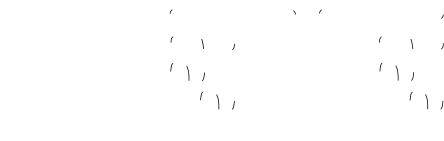
\includegraphics{media/chapters/04_temporal_tuning/04_04/haar_basis_overlay.pdf}%
	\caption[Visualisation of the orthonormal discrete Haar wavelets]{Visualisation of the orthonormal discrete Haar wavelets.
	\emph{Left:} Discrete basis transformation matrix $\mat W$ for $q = N = 32$. Blue is positive, red negative.
	\emph{Right:} Visualisation of the first eight rows in $\mat W$.
	Arrows correspond to the transitions mentioned in the text.
	}
	\label{fig:haar_basis}
\end{figure}

One particular set of discrete basis functions (\Cref{def:discrete_function_basis}) famous for allowing efficient state updates are the \emph{Haar wavelets} depicted in \Cref{fig:haar_basis} \citep{haar1910zur}.
A discrete Haar transformation $\mat W \vec u$ with $\mat W \in \mathbb{R}^{q \times N}$ can be computed in $\mathcal{O}(N)$ \citep{kaiser1998fast}, and the sliding spectrum can be updated in $\mathcal{O}(q)$ per sample.

To see this, assume that we store both our current state $\vec m_t$ and the last $N$ input samples $\vec u_t = (u_{t - N + 1}, \ldots, u_{t})$ in memory.
Sliding one of the discrete basis functions $W_i$ over $\vec u_t$, there are at most three samples in the input history that cross a transition point (arrows in the figure) and thus influence the value of $\vec m_t$.
Instead of re-convolving with $W_i$ and $\vec u_t$ in every time-step, we update $\vec m_t$ by accounting for the transitioning samples.

\subsubsection{Sliding Discrete Fourier Transform (\SDFT)}

Similar $\mathcal{O}(q)$ update algorithms can be obtained for the discrete Fourier and cosine basis (cf.~\Cref{sec:function_bases}), namely the sliding discrete Fourier (\SDFT; \cite{springer1991sliding,jacobsen2003sliding}) and cosine transformation (\SDCT; \cite{kober2004fast}).
Particularly, the \SDFT is given as (using real instead of complex coefficients):
\begin{align}
	&\begin{aligned}
		m^{2k - 1}_t &= m^{2k -1}_{t - 1} \cos(f_k) - m^{2k}_{t - 1} \sin(f_k) - u_{t - N} + u_{t}\,, \\
		m^{2k}_t &= m^{2k - 1}_{t - 1}    \sin(f_k) \, + m^{2k}_{t - 1} \cos(f_k) \,,
	\end{aligned} & \quad\quad \text{where} \quad f_k &= \frac{2 \pi k}{N} \,,
	\label{eqn:sdft}
\end{align}
where $m_t^{2k - 1}$ and $m_t^{2k}$ are the real and imaginary coefficients belonging to the frequency term $f_k$.
Note the similarity to a harmonic oscillator \LTI system with an additional delayed input, akin to our perfect continuous \LTI rectangle window in \Cref{lem:rectangle_window}.%
\footnote{Note that, in contrast to the Haar basis, computing the \SDFT does not require random access to the signal history $\vec u_t$. This drastically reduces the required memory bandwidth.}

\newcommand{\symLTI}{\includegraphics{media/chapters/04_temporal_tuning/04_04/sym_lti.pdf}}
\newcommand{\symSDT}{\includegraphics{media/chapters/04_temporal_tuning/04_04/sym_sdt.pdf}}
\newcommand{\symFIR}{\includegraphics{media/chapters/04_temporal_tuning/04_04/sym_fir.pdf}}

\begin{table}[p]
	\caption[Time and space complexity of different sliding transformations]{Time and space complexity of different sliding transformations.
	Memory requirements only take state retained between updates into account; we exclude constant matrices and filters.
	The column \enquote{window $N$} describes the relationship between $N$ and $q$ (typically $N \geq q$).
	Batch processing corresponds to computing the sliding window spectrum for every point in time for an entire recorded signal $\vec u$ of length $N$ in one go.
	Any sliding-window transformation has a \FIR representation and can always fall back to one of the algorithms in the first three rows.
	}
	\label{tbl:time_comparison}
	\small\sffamily
	{
	\centering
	\setlength{\tabcolsep}{8.75pt}
	\begin{tabular}{r l c c c c}
		\toprule
		& & \multicolumn{2}{c}{\textbf{Online} (per sample)} & \multicolumn{1}{c}{\textbf{Batch}} & \textbf{Window} $N$ \\
		\cmidrule(r){3-4}\cmidrule(r){5-5}\cmidrule{6-6}
		\emph{Basis} & \emph{Algorithm} & \emph{Time} & \emph{Memory} & \emph{Time} & \\
		\midrule
		\symLTI, \symSDT, \symFIR~Any & Na\"ive & $\mathcal{O}(qN)$ & $\mathcal{O}(N)$ & $\mathcal{O}(qN^2)$ & $\mathcal{O}(q)$ \\
		\cmidrule{2-6}
		    & FFT\textsuperscript{[1]} & / & / & $\mathcal{O}(qN \log(N))$ & $\mathcal{O}(q)$  \\
		\cmidrule{2-6}
		    & Gardner\textsuperscript{[2]} & $\mathcal{O}(q \log(N))$ & $\mathcal{O}(N \log(N))$ & / & $\mathcal{O}(q)$ \\
		\midrule
		\symLTI~LDN &
			ZOH\textsuperscript{[3]} & $\mathcal{O}(q^2)$ & $\mathcal{O}(q)$ & $\mathcal{O}(q^2 N)$ & $\mathcal{O}(q)$ \\
		\cmidrule{2-6}
		& Euler\textsuperscript{[4]} & $\mathcal{O}(q)$ & $\mathcal{O}(q)$ & $\mathcal{O}(qN)$ & $\approx \mathcal{O}(q^2)$ \\
		\midrule
		\symLTI~Mod. Fourier &
			ZOH\textsuperscript{[3]} & $\mathcal{O}(q^2)$ & $\mathcal{O}(q)$ & $\mathcal{O}(q^2N)$ & $\mathcal{O}(q)$ \\
		\cmidrule{2-6}
		& Euler\textsuperscript{[4]} & $\mathcal{O}(q)$ & $\mathcal{O}(q)$ & $\mathcal{O}(qN)$ & $\approx \mathcal{O}(q^{\frac{4}3})$ \\
		\midrule
		\symSDT~Fourier & SDFT\textsuperscript{[5]} & $\mathcal{O}(q)$ & $\mathcal{O}(N)$ & $\mathcal{O}(qN)$ & $\mathcal{O}(q)$ \\
		\midrule
		\symSDT~Cosine & SDCT\textsuperscript{[6]} & $\mathcal{O}(q)$ & $\mathcal{O}(N)$ & $\mathcal{O}(qN)$ & $\mathcal{O}(q)$ \\
		\midrule
		\symSDT~Haar & FHT\textsuperscript{[7]} & $\mathcal{O}(q)$ & $\mathcal{O}(N)$ & $\mathcal{O}(qN)$ & $\mathcal{O}(q)$ \\
		\bottomrule
	\end{tabular}\\[1em]
	}
	{\footnotesize
		\symLTI~Sliding transformation with a continuous \LTI state-space system of order $q$;
		\symSDT~Discrete sliding transformation with a fast update equation;
		\symFIR~Sliding transformation with a \FIR filter representation.
		[1] \cite{cooley1965algorithm};
		[2] \cite{gardner1995efficient};
		[3] See \cref{eqn:ldn_discretisation};
		[4] See \Cref{sec:ldn_computational_efficiency};
		[5] \cite{springer1991sliding}; \cite{jacobsen2003sliding};
		[6] \cite{kober2004fast};
		[7] \cite{kaiser1998fast}.
	}
\end{table}

\begin{figure}[p]
	\centering
	\includegraphics{media/chapters/04_temporal_tuning/04_04/sliding_trafo_sigmas.pdf}
	\caption[Comparing the orthogonality of different methods for generating sliding-window spectra]{
		Comparing the orthogonality of different methods for generating sliding-window spectra.
		Plotted is the sum $\Sigma$ of the normalised singular values of the system transformation matrices $\mat H$ for different $q$ (at $N = 1000$).
		When using sliding discrete transformations (\symSDT) or simple a set of arbitrary \FIR filters (\symFIR), it holds $\Sigma = q$.
		The quality of the basis generated by the \LDN and the modified Fourier system (\symLTI) is suboptimal.
	Note that $\Sigma \approx 0.88q$ for the modified Fourier basis (for odd $q$); the slope of $88\%$ is close to the percentage to which the individual state dimensions have been slowed down ($90\%$).
	}
	\label{fig:sliding_trafo_sigmas}
\end{figure}

%Crucially, since the truncated Fourier basis possesses perfect low-pass characteristics with cutoff frequency $\hat f$ at $2 \hat f = q - 1$, we require, by the Nyquist-Shannon sampling theorem \citep{shannon1949communication}, $q$ samples to cover a window period $\theta$.
%Correspondingly, we only need to store $q$ samples in memory for implementing the delay line.%
%\footnote{In practice, some headroom is required, i.e., we should have $N > q$ samples per window period; this way, the downsampler can be simpler. This does not change the asymptotic complexity since $N$ can be linear in $q$.}
%Of course, this requires that the input is downsampled to $q$ samples per $\theta$.
%Luckily, down- and upsampling are well studied aspects of digital signal processing with efficient solutions \citep[Chapter~4]{oppenheim2009discretetime}.
%
%\begin{figure}
%	\centering
%	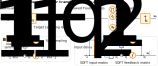
\includegraphics{media/chapters/04_temporal_tuning/04_04/optimal_sliding_window_trafo.pdf}
%	\caption[A sliding Fourier transform with optimal memory and time requirements]{A sliding Fourier transform with optimal memory and time requirements. This system performs a sliding basis transformation while not requiring more than $\mathcal{O}(q)$ space and $\mathcal{O}(qN)$ time per sliding window period $\theta$, where $N$ can be on the order of $q$.
%	\textbf{(A)} The input signal is downsampled to (more than) $q$ samples per $\theta$ and convolved with the windowed Fourier basis. If so desired, the $q$ signals can be upsampled to match the original rate.
%	This may be important if there are subsequent nonlinear transformations, as in the LMU.
%	\textbf{(B)} In the simplest case, a downsampler is a low-pass filter passing on a fraction of the input samples.
%	\textbf{(C)} Convolution with the windowed Fourier basis can be computed efficiently using \cref{eqn:sdft}; these equations describe an LTI system with an input delay.
%	}
%	\label{fig:optimal_sliding_window_trafo}
%\end{figure}
%
%Correspondingly, as is depicted in \Cref{fig:optimal_sliding_window_trafo}, we can envision a system with $\mathcal{O}(q)$ memory complexity and a $\mathcal{O}(qN)$ time complexity for processing a single time-window of length $\theta$ \emph{online}, where $N \geq q$ may be linear in $q$.
%Depending on the quality of the downsampler, the system implements the windowed Fourier transforma with little distortion.
%The main downside of such a system---aside from the more complex implementation and larger constant factors---is that resampling introduces a small delay.


\subsection{Experiments}
\label{sec:lmu_experiments}

So far, we have seen several alternatives to the \LDN system used in the Legendre Memory Unit.
As is summarised in \Cref{tbl:time_comparison}, these systems can be implemented in different ways, each with different characteristics in terms of time and space complexity, and different degrees to which they realise an orthogonal function basis (\Cref{fig:sliding_trafo_sigmas}).

To explore how well these systems actually perform in a neural network context, we repeat two experiments from the original \LMU paper \citep{voelker2019lmu}; specifically, the psMNIST and Mackey-Glass tasks.
Our goal is to explore in how far changing the sliding-window transformation affects the performance of the \LMU in comparison to the \LDN variant.
%Readers interested in studies comparing the \LMU to other neural network architectures are kindly referred to the beginning of this section, where we provide several references.

Our results indicate that the basis choice has a significant, but small effect on the system performance.
The power of the \LMU architecture stems from using a \emph{fixed} and \emph{orthogonal} temporal projection; the particular shape and quality of this projection are secondary.
Practitioners should select a transformation from \Cref{tbl:time_comparison} that suits their particular constraints.

\subsubsection{psMNIST}

\begin{figure}
	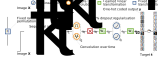
\includegraphics{media/chapters/04_temporal_tuning/04_04/psmnist_overview_overlay.pdf}%
	\kern-158mm\includegraphics{media/chapters/04_temporal_tuning/04_04/psmnist_overview.pdf}%
	\caption[Overview of the psMNIST task and our network architecture]{Overview of the psMNIST task and our network architecture.
	Input images are randomly permuted and serialised into a stream of pixels presented over time.
	After all $N = 784$ pixels have been fed into the network, the network must output the correct one-hot coded classification.
	In our particular case $q = 468$ and $n = 346$ for a total of \num{166000} weights.}
	\label{fig:psmnist_overview}
\end{figure}

The MNIST dataset \citep{lecun1998gradientbased} contains $28 \times 28$ pixel greyscale images of hand-written digits between zero and nine.
The task is to classify the digits; state-of-the-art classification accuracies are above $99\%$ \citep{baldominos2019survey}.

The permuted sequential MNIST (psMNIST) task has originally been proposed by \citet{le2015simple}.
The idea is to turn the MNIST dataset into a benchmark for the memory capacity of recurrent neural networks.
Specifically, each image is treated as a sequence $\vec u$ of $N = 784$ pixels.
Each pixel is fed one-by-one into the network in consecutive timesteps.
Once the final sample has been processed, the system must correctly classify the digit.
To eliminate spatial correlations in the input, a random but fixed permutation $\pi$ is applied to the samples (cf.~\Cref{fig:psmnist_overview}).
The input signal is thus of the form $\vec u = (u_{\pi(1)}, \ldots, u_{\pi(784)})$.

\paragraph{Additional constraints}
The psMNIST task as described above is slightly under-defined.
Specifically, two additional constraints should be met.
First, the network should use less state memory than is required to just store the whole image \citep{voelker2019lmu}.
Second, the network should support \emph{serial execution} \citep{chandar2019nonsaturating}.
In other words, the network must produce correct classifications over time, even if multiple input signals are concatenated.

Implementing temporal convolution as \FIR filters of length $N$ (cf.~\Cref{sec:lmu}) intrinsically fulfils the serial execution constraint, but violates the memory constraint.
Each filter requires access to the past $N$ samples; we essentially just compute the inner product between each of the $q$ \FIR filters and the input.
The point of using the \LDN or modified Fourier system impulse response is that the same convolution can be performed by an \LTI system of order (and thus memory) $q < N$ within the recurrent \LRGF \LMU network.%
\footnote{Note that both the LDN and modified Fourier system impulse response produce ringing artefacts that extend beyond the first $N$ samples (cf.~\Cref{fig:modified_euler_stress}), that is, there is some interaction between two consecutively presented input images.
We ignore this to be consistent with the way the psMNIST task is typically evaluated in the literature.
However, we take ringing into account in the Mackey-Glass experiment.}
Therefore, the results for our $\mathcal{O}(N)$ memory transformations should be taken with a grain of salt.

\paragraph{Methods}
Our network architecture is similar to the setup used by \citet{voelker2019lmu}.
We provide an overview of the model in \Cref{fig:psmnist_overview}; the code describing the network can be found in \Cref{app:lmu_code}.
We apply a set of $q = 468$ \FIR filters to the $N = 784$ input samples.
The filter output is passed through a 50\% dropout layer for regularisation \citep{hinton2012improving}, followed by $n = 346$ \ReLU neurons that nonlinearly processes the temporal representation.
The neural activities are linearly projected onto a one-hot coded output.
Note that $q = 468$ is motivated by the amount of memory used by \citet{chandar2019nonsaturating}.

As is customary, we split the MNIST dataset into $50\,000$ training and $10\,000$ validation samples.
We use a categorical cross-entropy loss function and an Adam optimiser \citep{kingma2015adam} with default parameters over $100$ epochs at a batch size of $100$.
The reported test errors are computed for the epoch with the smallest validation error.
For $q = 468$ the number of trainable parameters is $\approx\num{166000}$.
Per default, the \FIR filters are fixed and initialised with one of the previously discussed discretised basis transformations with window length $N = 786$ (i.e., the number of pixels).
The \LTI systems are discretised using zero-order hold.

As a point of comparison, we repeat the experiments with randomly initialised \FIR filters, as well as enabled learning for the \FIR filter matrices.
Learning the \FIR filters adds another \num{350000} parameters and is supposed to test in how far our original transformations are optimal.

\begin{figure}
\centering
\includegraphics{media/chapters/04_temporal_tuning/04_04/psmnist_results.pdf}
\caption[Classification accuracies for the psMNIST dataset using different sliding-window transformations]{Classification accuracies for the psMNIST dataset using different sliding-window transformations.
Depicted are standard box-plots over $101$ trials for each basis, each with a different random permutation $\pi$ and weight initialisations. Box corresponds to the first and third quartile; whiskers are the minimum/maximum after outlier rejection; outliers are depicted as circles.
Dashed black line is the mean, notches correspond to the bootstrapped $95\%$ confidence interval.
Numerical values and significance levels are provided in \Cref{tbl:psmnist_results}.
Symbols correspond to possible algorithms from \Cref{tbl:time_comparison}.
}
\label{fig:psmnist_results}
\end{figure}

\begin{table}
	\caption[Test accuracies for the psMNIST experiment]{Test accuracies for the psMNIST experiment for $q = 468$. Data over $n = 101$ trials and $100$ epochs. Q1 and Q3 are the 25- and 75-percentile, respectively. The best three results are highlighted in each column (darker colours are better).}
	\label{tbl:psmnist_results}
	\centering\small\sffamily
	\setlength{\tabcolsep}{7.25pt}
	\begin{tabular}{r  r r r r  r r r r}
	\toprule
	& \multicolumn{4}{c}{{\color{skyblue1}$\blacksquare$} \textbf{Fixed convolution}}
	& \multicolumn{4}{c}{{\color{aluminium2}$\blacksquare$} \textbf{Learned convolution}} \\
	\cmidrule(r){2-5}\cmidrule(l){6-9}
	\emph{Basis} &
	\emph{Mean} &
	\emph{Median} &
	\emph{Q1} &
	\emph{Q3} &
	\emph{Mean} &
	\emph{Median} &
	\emph{Q1} &
	\emph{Q3} \\
	\midrule
		\symLTI~LDN &
			98.49\% &
			98.48\% &
			98.44\% &
			98.55\% &
			 \cellcolor{CornflowerBlue!25}{98.23\%} &
			98.22\% &
			 \cellcolor{CornflowerBlue!25}{98.16\%} &
			 \cellcolor{CornflowerBlue!25}{98.30\%} \\
			\symLTI~Mod.~Fourier &
			98.53\% &
			 \cellcolor{CornflowerBlue!50}{98.54\%} &
			 \cellcolor{CornflowerBlue!25}{98.48\%} &
			98.58\% &
			 \cellcolor{CornflowerBlue!75}{98.24\%} &
			 \cellcolor{CornflowerBlue!50}{98.24\%} &
			 \cellcolor{CornflowerBlue!75}{98.18\%} &
			 \cellcolor{CornflowerBlue!50}{98.31\%} \\
			\symSDT~Fourier &
			 \cellcolor{CornflowerBlue!75}{98.56\%} &
			 \cellcolor{CornflowerBlue!75}{98.56\%} &
			 \cellcolor{CornflowerBlue!75}{98.51\%} &
			 \cellcolor{CornflowerBlue!75}{98.62\%} &
			98.21\% &
			98.21\% &
			98.13\% &
			 \cellcolor{CornflowerBlue!25}{98.30\%} \\
			\symSDT~Cosine &
			 \cellcolor{CornflowerBlue!50}{98.54\%} &
			 \cellcolor{CornflowerBlue!50}{98.54\%} &
			 \cellcolor{CornflowerBlue!50}{98.49\%} &
			 \cellcolor{CornflowerBlue!50}{98.60\%} &
			98.22\% &
			98.22\% &
			 \cellcolor{CornflowerBlue!25}{98.16\%} &
			98.29\% \\
			\symSDT~Haar &
			98.47\% &
			98.46\% &
			98.40\% &
			98.53\% &
			98.22\% &
			98.22\% &
			98.14\% &
			98.29\% \\
			\symFIR~DLOP &
			 \cellcolor{CornflowerBlue!50}{98.54\%} &
			 \cellcolor{CornflowerBlue!50}{98.54\%} &
			 \cellcolor{CornflowerBlue!25}{98.48\%} &
			 \cellcolor{CornflowerBlue!50}{98.60\%} &
			 \cellcolor{CornflowerBlue!25}{98.23\%} &
			 \cellcolor{CornflowerBlue!25}{98.23\%} &
			98.14\% &
			 \cellcolor{CornflowerBlue!25}{98.30\%} \\
			\symFIR~Random &
			98.11\% &
			98.13\% &
			98.05\% &
			98.19\% &
			 \cellcolor{CornflowerBlue!75}{98.24\%} &
			 \cellcolor{CornflowerBlue!75}{98.25\%} &
			 \cellcolor{CornflowerBlue!50}{98.17\%} &
			 \cellcolor{CornflowerBlue!75}{98.32\%} \\
	\bottomrule
	\end{tabular}
\end{table}

\begin{table}
	\newcommand{\sigA}{\ensuremath{\cdot}}
	\newcommand{\sigB}{\ensuremath{\bullet\bullet}}
	\newcommand{\sigC}{\ensuremath{\bullet\!\bullet\!\bullet}}
	\caption[Statistical significance of the psMNiST test accuracies]{Statistical significance of the psMNIST test accuracies. The given significance levels are based on a two-sided Kolmogorov-Smirnov test; $\sigA \correspondsTo p < 0.05$, $\sigB \correspondsTo p < 0.01$, $\sigC \correspondsTo p < 0.001$.}
	\label{tbl:psmnist_significance}
	\centering\small\sffamily
	\setlength{\tabcolsep}{6.2pt}
	\begin{tabular}{r r  c c c c c c c  c c c c c c c}
	\toprule
	& & \multicolumn{7}{c}{{\color{skyblue1}$\blacksquare$} \textbf{Fixed convolution}}
	& \multicolumn{7}{c}{{\color{aluminium2}$\blacksquare$} \textbf{Learned convolution}} \\
	\cmidrule(r){3-9}\cmidrule(l){10-16}
	\emph{Basis} & & (1) & (2) & (3) & (4) & (5) & (6) & (7)  & (1) & (2) & (3) & (4) & (5) & (6) & (7) \\
	\midrule
	\symLTI~LDN & (1) &
		 &
		\sigC &
		\sigC &
		\sigC &
		 &
		\sigB &
		\sigC &
		 &
		 &
		 &
		 &
		 &
		 &
		 \\
		\symLTI~Mod.~Fourier & (2) &
		\sigC &
		 &
		 &
		 &
		\sigC &
		 &
		\sigC &
		 &
		 &
		 &
		 &
		 &
		 &
		 \\
		\symSDT~Fourier & (3) &
		\sigC &
		 &
		 &
		 &
		\sigC &
		 &
		\sigC &
		 &
		 &
		 &
		 &
		 &
		 &
		 \\
		\symSDT~Cosine & (4) &
		\sigC &
		 &
		 &
		 &
		\sigC &
		 &
		\sigC &
		 &
		 &
		 &
		 &
		 &
		 &
		 \\
		\symSDT~Haar & (5) &
		 &
		\sigC &
		\sigC &
		\sigC &
		 &
		\sigC &
		\sigC &
		 &
		 &
		 &
		 &
		 &
		 &
		 \\
		\symFIR~DLOP & (6) &
		\sigB &
		 &
		 &
		 &
		\sigC &
		 &
		\sigC &
		 &
		 &
		 &
		 &
		 &
		 &
		 \\
		\symFIR~Random & (7) &
		\sigC &
		\sigC &
		\sigC &
		\sigC &
		\sigC &
		\sigC &
		 &
		 &
		 &
		 &
		 &
		 &
		 &
		 \\
	\bottomrule
	\end{tabular}
\end{table}

\paragraph{Results}
Results are depicted in \Cref{fig:psmnist_results} and \Cref{tbl:psmnist_results,tbl:psmnist_significance}; learning curves are provided in \Cref{fig:lmu_trajs}.
The modified Fourier, Fourier, cosine and discrete Legendre (\DLOP; \Cref{sec:function_bases}) basis outperform the \LDN and Haar wavelets slightly but significantly.
The \LDN result is state-of-the art for the psMNIST task at about $98.5\%$ accuracy \citep{chilkuri2021parallelizing}.
There is no significant difference between initialisations when learning the convolution; enabling learning on the \FIR filters always results in the same, substantially worse performance.

\paragraph{Discussion}
Learned convolutions performing worse is likely a result of the increased parameter count and overfitting to the training data (cf.~\Cref{fig:lmu_trajs}).
Visualising the learned \FIR filters (data not shown), we find that they do not differ substantially from their original initialisation.
This suggests that our orthogonal transformations are locally optimal.

Thinking about the \FIR filter matrix $\mat H$ purely in terms of a projection $\mat H \vec u$, it is unclear why our systematic bases work better than a random initialisation---after all, this results in an (almost) orthogonal projection as well.
There is a history of successfully applying orthogonal basis transformations such as the discrete Cosine or Haar transform to the MNIST dataset for spatial decorrelation \citep{baldominos2019survey}.
However, these experiments are without pixel permutation; with permutation, spatial decorrelation is an unlikely explanation.

One hint at the worse performance of the random initialisation is our \enquote{orthogonality measure} $\Sigma$ (that is, the sum of the normalised singular values).
For the random \FIR filters $\Sigma$ is only about $0.5q$, while we reach higher $\Sigma$ for our other bases (cf.~\Cref{fig:sliding_trafo_sigmas}).


\subsubsection{Mackey-Glass}

\begin{figure}
	\includegraphics{media/chapters/04_temporal_tuning/04_04/mackey_glass_system.pdf}
	\caption[Visualisation of the Mackey-Glass system]{Visualisation of the Mackey-Glass system as used in our benchmark task.
	Left plot shows a short segment of the state evolution, the right plot a 2D delay embedding (delay of $10$ samples).
%	\textbf{(A)}~For $\tau \geq 17$ the system behaves mildly chaotically. \textbf{(B)}~For $\tau = 30$ the system is fully chaotic.
	}
	\label{fig:mackey_glass_system}
\end{figure}

The Mackey-Glass dynamical system \citep{mackey1977oscillation} is a popular benchmark for time-series prediction \citep[cf.][Section 4.3.1]{mendel2017uncertain}.
The goal is to predict the time-course of the following differential equation (cf.~\Cref{fig:mackey_glass_system}).
\begin{align*}
	\dot{\vec u}(t) &= \frac{a u(t - \tau)}{1 + u(t - \tau)^{10}} - b u(t) \quad\quad \text{for} \quad t \geq 0\,,
\end{align*}
where $a = 0.2$, $b = 1.2$.
For $t < 0$ we assume that the state variable $u(t)$ is a Gaussian process with mean $\mu = 1.2$ and standard-deviation $\sigma = 1$.
Notably, the system behaves chaotically if $\tau \geq 17$; that is, small perturbations to the initial state can lead to dramatically different state trajectories.
This makes predicting the system particularly hard.
For our experiment, we construct a network that attempts to predict the time-course of the discretised Mackey-Glass system with $\tau = 30$ for the next fifteen state samples $u_{t + 1}, \ldots, u_{t + 15}$ given the recent state history.

\paragraph{Dataset}
For our experiments, we choose $\tau = 30$.
As a training dataset we generate $400$ Mackey-Glass state trajectories consisting of \num{10000} samples at $\Delta t = 1$ using a fourth order Runge-Kutta integrator; the trajectories are normalised to mean zero and standard deviation one.
All trajectories are different due to the stochasticity of the initial $u(t)$ for $t < 0$.

We randomly extract 100 input sequences of length $117$ followed by a target sequence of length 15 from each trajectory; this results in 40\,000 training samples. We similarly generate \num{10000} validation and \num{10000} test samples.
Training, validation, and test samples are all taken from separately generated trajectories.
The sample length $117$ corresponds to the absolute width of the combined \FIR filters in our network; as is illustrated in \Cref{fig:mackey_glass_overview_overlay_b}, only the last $37$ samples are effectively taken into account for the prediction.

\begin{figure}
	\includegraphics{media/chapters/04_temporal_tuning/04_04/mackey_glass_overview.pdf}%
	\kern-158mm\includegraphics{media/chapters/04_temporal_tuning/04_04/mackey_glass_overview_overlay.pdf}\\[0.25cm]
	{\phantomsubcaption\label{fig:mackey_glass_overview_overlay_a}}%
	{\phantomsubcaption\label{fig:mackey_glass_overview_overlay_b}}%
	\caption[Overview of the Mackey-Glass prediction network and dataset]{
		Overview of the Mackey-Glass prediction network and dataset.
		\textbf{(A)} Samples $u_t$ fed into the network pass a series of four \LMU layers (here depicted as \FIR \LMUpl); the output is a prediction $\vec{\hat y}_t$ of the next fifteen samples $u_{t + 1}, \ldots, u_{t + 15}$.
		Every sample fed into the network immediately updates the prediction in the output.
		When using the \LDN or the modified Fourier system as a sliding transformation, the \FIR \LMUpl can of course be replaced with a corresponding recurrent \LRGF \LMU.
		\textbf{(B)} Exemplary input-target pair for $\tau = 17$.
		The absolute window of the \FIR filters in our network amounts to $117$ samples; samples older than this cannot \emph{possibly} affect the output. However, only the last $37$ samples \emph{effectively} influence the system.
		The longer absolute window ensures that we account for ringing artefacts in the \LDN and modified Fourier system (cf.~\Cref{fig:lmu_mackey_glass_filters}).
	}
	\label{fig:mackey_glass}
\end{figure}

\paragraph{Methods}
Our neural network architecture is inspired by \citet{voelker2019lmu} and depicted in \Cref{fig:mackey_glass}.
The relevant code may be found in \Cref{app:lmu_code}.

There are four cascading \LMU layers; the last three layers consist of ten stacked sliding-window transformations each.
In contrast to the previous experiment, each transformation uses small $q$ with $N = q$.
Note that a sliding-window transformation with $q = N$ is lossless, and that the linear readout weights can theoretically decode the state in terms of any other basis.%
\footnote{$q = N$ is a good use-case for an efficient sliding-window spectrum (\Cref{sec:efficient_sliding_window}).
This requires $2q$ memory and less computation than the \LDN system---we cannot use an efficient Euler update for $q = N$ (\Cref{sec:ldn_computational_efficiency}).}
Specifically, the first \LMU layer uses $q_1 = N_1 = 17$, the second and third $q_{23} = N_{23} = 9$, and the final layer $q_{4} = N_4 = 5$.
Assuming that our sliding-transformation implements a perfect rectangle window, this results in the aforementioned \emph{effective} combined window width of $37$.%
\footnote{Specifically, $37 = N_1 + N_2 + N_3 + N_4 - 3$. Each layer \enquote{consumes} $N_i - 1$ samples, and one additional sample is required to obtain a single output sample. See also our discussion in \Cref{app:lmu_code}.}
The absolute window width stems from the impulse response of the \LDN and modified Fourier system technically extending beyond $N_i$.
For good measure, we therefore extend the \FIR filters to be three times as long as the actual window width.

As in the previous experiment, we compare fixed convolutions, including random initialisations, to a version of the network where the convolutions are initialised in the same way, but then trained during training.
Note that we do not train the extended filters.
The total number of parameters is $2750$; another $476$ parameters are added if the convolutions are trained.

We train the network for $100$ epochs with a batch size of $100$ using a standard Adam optimiser.
The final test error is computed for the parameters in the epoch with the smallest validation error.
Our training loss is the \MSE, we report the \NRMSE.
Note that our results are not directly comparable to those in the literature due to using a different $\tau$ and normalisation of the Mackey-Glass dataset.
Our goal is merely to compare different \LMU variants.

\paragraph{Results}

\begin{figure}[p]
\centering
\includegraphics{media/chapters/04_temporal_tuning/04_04/mackey_glass_results.pdf}
\caption[Prediction errors for the Mackey-Glass dataset using different sliding-window transformations]{Prediction errors for the Mackey-Glass dataset using different sliding-window transformations. See \Cref{fig:psmnist_results} for a description of the plot.
Numerical values are given in \Cref{tbl:mackey_glass_results}.}
\label{fig:mackey_glass_results1}
\end{figure}

\begin{table}[p]
	\newcommand{\sigA}{\ensuremath{\cdot}}
	\newcommand{\sigB}{\ensuremath{\bullet\bullet}}
	\newcommand{\sigC}{\ensuremath{\bullet\!\bullet\!\bullet}}
	\caption[Prediction errors and statistical analysis for the Mackey-Glass dataset]{Prediction errors and statistical analysis for the Mackey-Glass dataset. Data over $101$ trials after $100$ epochs of training. See \Cref{tbl:psmnist_results,tbl:psmnist_significance} for a description.
	The given significance levels are based on a two-sided Kolmogorov-Smirnov test; $\sigA \correspondsTo p < 0.05$, $\sigB \correspondsTo p < 0.01$, $\sigC \correspondsTo p < 0.001$.
	}
	\label{tbl:mackey_glass_results}
	\centering\small\sffamily
	\setlength{\tabcolsep}{8.79pt}
	\begin{tabular}{r  r r r r  r r r r}
	\toprule
	& \multicolumn{4}{c}{{\color{skyblue1}$\blacksquare$} \textbf{Fixed convolution}}
	& \multicolumn{4}{c}{{\color{aluminium2}$\blacksquare$} \textbf{Learned convolution}} \\
	\cmidrule(r){2-5}\cmidrule(l){6-9}
	\emph{Basis} &
	\emph{Mean} &
	\emph{Median} &
	\emph{Q1} &
	\emph{Q3} &
	\emph{Mean} &
	\emph{Median} &
	\emph{Q1} &
	\emph{Q3} \\
	\midrule
	\symLTI~LDN &
	 \cellcolor{CornflowerBlue!75}{3.63\%} &
	 \cellcolor{CornflowerBlue!75}{3.43\%} &
	 \cellcolor{CornflowerBlue!75}{2.98\%} &
	 \cellcolor{CornflowerBlue!75}{4.22\%} &
	 \cellcolor{CornflowerBlue!75}{3.80\%} &
	 \cellcolor{CornflowerBlue!50}{3.64\%} &
	 \cellcolor{CornflowerBlue!75}{3.09\%} &
	 \cellcolor{CornflowerBlue!25}{4.37\%} \\
	\symLTI~Mod.~Fourier &
	4.38\% &
	4.26\% &
	3.61\% &
	4.78\% &
	3.89\% &
	3.70\% &
	 \cellcolor{CornflowerBlue!50}{3.15\%} &
	4.39\% \\
	\symSDT~Fourier &
	4.21\% &
	3.95\% &
	3.42\% &
	4.58\% &
	3.93\% &
	3.83\% &
	3.32\% &
	4.52\% \\
	\symSDT~Cosine &
	 \cellcolor{CornflowerBlue!25}{3.96\%} &
	 \cellcolor{CornflowerBlue!50}{3.64\%} &
	 \cellcolor{CornflowerBlue!25}{3.25\%} &
	 \cellcolor{CornflowerBlue!50}{4.26\%} &
	 \cellcolor{CornflowerBlue!75}{3.80\%} &
	 \cellcolor{CornflowerBlue!75}{3.59\%} &
	3.22\% &
	 \cellcolor{CornflowerBlue!50}{4.33\%} \\
	\symSDT~Haar &
	4.01\% &
	3.82\% &
	3.29\% &
	4.57\% &
	3.95\% &
	3.82\% &
	3.22\% &
	4.58\% \\
	\symFIR~DLOP &
	 \cellcolor{CornflowerBlue!50}{3.90\%} &
	 \cellcolor{CornflowerBlue!25}{3.75\%} &
	 \cellcolor{CornflowerBlue!50}{3.17\%} &
	 \cellcolor{CornflowerBlue!25}{4.42\%} &
	 \cellcolor{CornflowerBlue!25}{3.86\%} &
	 \cellcolor{CornflowerBlue!25}{3.65\%} &
	 \cellcolor{CornflowerBlue!25}{3.16\%} &
	 \cellcolor{CornflowerBlue!75}{4.32\%} \\
	\symFIR~Random &
	5.38\% &
	5.12\% &
	4.38\% &
	6.15\% &
	4.04\% &
	3.87\% &
	3.30\% &
	4.51\% \\
	\symFIR~Identity &
	5.21\% &
	5.03\% &
	4.38\% &
	5.81\% &
	4.04\% &
	3.87\% &
	3.31\% &
	4.67\% \\
	\bottomrule
	\end{tabular}\\[10pt]
	\centering\small\sffamily
	\setlength{\tabcolsep}{4.75pt}
	\begin{tabular}{r r  c c c c c c c c  c c c c c c c c}
	\toprule
	& & \multicolumn{8}{c}{{\color{skyblue1}$\blacksquare$} \textbf{Fixed convolution}}
	& \multicolumn{8}{c}{{\color{aluminium2}$\blacksquare$} \textbf{Learned convolution}} \\
	\cmidrule(r){3-10}\cmidrule(l){11-18}
	\emph{Basis} & & (1) & (2) & (3) & (4) & (5) & (6) & (7) & (8)  & (1) & (2) & (3) & (4) & (5) & (6) & (7) & (8) \\
	\midrule
	\symLTI~LDN & (1) &
	 &
	\sigC &
	\sigC &
	 &
	\sigB &
	\sigA &
	\sigC &
	\sigC &
	 &
	 &
	 &
	 &
	 &
	 &
	 &
	 \\
	\symLTI~Mod.~Fourier & (2) &
	\sigC &
	 &
	 &
	\sigB &
	 &
	\sigA &
	\sigC &
	\sigC &
	 &
	 &
	 &
	 &
	 &
	 &
	 &
	 \\
	\symSDT~Fourier & (3) &
	\sigC &
	 &
	 &
	 &
	 &
	 &
	\sigC &
	\sigC &
	 &
	 &
	 &
	 &
	 &
	 &
	 &
	 \\
	\symSDT~Cosine & (4) &
	 &
	\sigB &
	 &
	 &
	 &
	 &
	\sigC &
	\sigC &
	 &
	 &
	 &
	 &
	 &
	 &
	 &
	 \\
	\symSDT~Haar & (5) &
	\sigB &
	 &
	 &
	 &
	 &
	 &
	\sigC &
	\sigC &
	 &
	 &
	 &
	 &
	 &
	 &
	 &
	 \\
	\symFIR~DLOP & (6) &
	\sigA &
	\sigA &
	 &
	 &
	 &
	 &
	\sigC &
	\sigC &
	 &
	 &
	 &
	 &
	 &
	 &
	 &
	 \\
	\symFIR~Random & (7) &
	\sigC &
	\sigC &
	\sigC &
	\sigC &
	\sigC &
	\sigC &
	 &
	 &
	 &
	 &
	 &
	 &
	 &
	 &
	 &
	 \\
	\symFIR~Identity & (8) &
	\sigC &
	\sigC &
	\sigC &
	\sigC &
	\sigC &
	\sigC &
	 &
	 &
	 &
	 &
	 &
	 &
	 &
	 &
	 &
	 \\
	\bottomrule
	\end{tabular}
\end{table}

Results are given in \Cref{fig:mackey_glass_results1} and \Cref{tbl:mackey_glass_results}; see \Cref{fig:lmu_trajs} for learning curves.
Overall, all bases perform similarly, with the \LDN outperforming the Fourier and modified Fourier bases.
The modified Fourier basis performs worst.
The random and identity initialisations result in by far the highest errors, and the \LDN, cosine, and \DLOP filters result in the lowest error.
Learning the convolution closes the performance-gap between the bases.

\paragraph{Discussion}
The cause of the unfavourable performance of the modified Fourier basis is unclear.
We can rule out the ringing artefacts (cf.~\Cref{fig:lmu_mackey_glass_filters})---the performance gap remains after forcing a perfect rectangle window (see \Cref{fig:mackey_glass_ne} and \Cref{tbl:mackey_glass_results_ne}); however, the superiority of the \LDN over the other bases vanishes in this case.

A possible culprit is that the best-performing bases (i.e., the \LDN, \DLOP, and cosine basis) are aperiodic, and that even the unmodified Fourier basis performs slightly worse than the other bases.
Using a sub-optimal Fourier basis may thus further reduce the performance to the level observed here.
However, a more detailed analysis is required.

Overall, our results indicate that the basis choice is secondary, as long at it is not random or an identity basis.
Using fixed orthogonal temporal convolutions can greatly reduce the number of trainable parameters without sacrificing performance.
The particular architecture to choose (e.g., \FIR or \LRGF \LMU), or whether to rely on an order $q$ \LTI system instead of an efficient sliding-window transformation depends on the particular application.
Limiting constraints are the sampling rate (determining whether a fast Euler update is possible), available memory, as well as latency requirements (i.e., whether to use batch or online processing).
